\documentclass{article}

% NeurIPS 2026 double-blind workshop submission.
\usepackage[dblblindworkshop]{neurips_2026}
\workshoptitle{Structured Reasoning for Interpretability and Control (StRICt)}

\usepackage[T1]{fontenc}
\usepackage[utf8]{inputenc}
\usepackage{courier}
\usepackage{hyperref}
\hypersetup{hidelinks,hypertexnames=false}
\usepackage{url}
\usepackage{microtype}
\usepackage{graphicx}
\usepackage{booktabs}
\usepackage{amsmath}
\usepackage{amssymb}
\usepackage{xcolor}
\definecolor{PaperOcean}{HTML}{3C8FA4}
\definecolor{PaperCoral}{HTML}{C96F5F}
\definecolor{PaperSand}{HTML}{D8C58D}
\definecolor{PaperInk}{HTML}{202A33}
\definecolor{PaperGrid}{HTML}{DCE4E7}
\usepackage{tikz}
\usetikzlibrary{shapes,arrows.meta,positioning,calc,fit,backgrounds}
\usepackage{placeins}
\usepackage{float}
\def\UrlBreaks{\do\/\do-\do_}

\title{Redirect, Escalate, or Abstain?\\Selective Recovery for Code Agents}

\author{Anonymous Author(s)}

\begin{document}
\maketitle

\begin{abstract}
Recovery prompts are usually treated as harmless retries.  We instead formulate
code-agent recovery as a selective control problem: from the observable history,
a controller must decide whether to issue a lightweight redirect, escalate to
richer execution evidence, or abstain.  We ground this formulation in 143 failed
SWE-bench Verified trajectories and more than 1,400 controlled next-action
responses spanning four operational failure categories and nine models.  The
audit reveals an asymmetric evidence pattern.  The aggregate gain of
category-matched redirects is +0.50 on a 0--3 regex proxy, but falls to 0.00
when type-lexical relevance is removed; a blinded LLM judge gives +0.14 on 37
paired responses with an interval containing zero.  By contrast, 10 of 12
off-diagonal redirect--category pairs fall below same-instance control on the
full proxy, and 11 of 12 do so without relevance.  These results do not
establish software repair.  They show why recovery should optimize
intervention utility rather than category accuracy alone, validate progress
after acting, and preserve abstention under uncertainty.
\end{abstract}

%% ============================================================
%% SECTION 1: INTRODUCTION
%% ============================================================
\section{Introduction}

Helping a failing code agent is not always helpful.  Once an agent exposes an
error, a recovery system can redirect its behavior, request additional evidence,
restart part of the search, or leave the trajectory untouched.  These are
control actions with different costs and failure modes, not interchangeable
wordings of a generic ``try again'' prompt.  An always-intervene policy can
therefore compound the error it was intended to correct.

A concrete result illustrates the risk.  In our controlled study, a
test-guided instruction applied to localization failures scores 0.87 on a 0--3
next-action proxy, below the 1.70 unscaffolded control.  The instruction is
reasonable in isolation, yet it presupposes that test execution is the missing
behavior.  When the actual bottleneck is search, this additional directive can
displace a more useful action.  Recovery quality thus depends on the
interaction between an observed trajectory and an intervention, not on the
intervention in isolation.

This interaction is easy to miss because failed trajectories are structurally
heterogeneous.  An agent repeating a stale \texttt{str\_replace} command is in a
different state from one editing a gold-patch file with an incorrect fix.  A
third agent may still be searching outside the relevant files.  These histories
can all end in failure while supporting different control decisions.  The key
question is consequently not only \emph{what failed}, but \emph{whether a
particular intervention has positive expected value given the evidence
available now}.

We formalize this question as \emph{selective recovery}
(\S\ref{sec:formulation}).  A controller observes only the trajectory prefix
available at decision time and chooses among a lightweight behavioral redirect,
an evidence-seeking escalation, and abstention.  The decision objective is the
incremental task utility relative to leaving the agent alone, including the
cost and potential harm of intervention.  This view separates three errors that
an aggregate recovery score otherwise conflates: misdiagnosing the state,
choosing an unsuitable action, and failing to verify the resulting progress.

We ground the formulation in 143 failed SWE-bench Verified trajectories
\citep{jimenez2024swebench}.  Four operational categories summarize edit-tool
failure, localization, applied-but-incorrect patches, and residual plan-level
failure.  We then audit more than 1,400 stored next-action responses under
matched, mismatched, held-out-selection, and cross-model conditions.  The
controlled data are oracle-context diagnostics rather than a deployed
controller, but they reveal the asymmetry that motivates selective recovery:
large apparent matched gains are evaluator-sensitive, whereas negative transfer
is more persistent across proxy specifications.  Figure~\ref{fig:framework}
summarizes the resulting design.

Our contributions are:
\begin{itemize}
\setlength{\itemsep}{0pt}
\item We formulate code-agent recovery as risk-sensitive selection among
redirect, evidence escalation, and abstention, with intervention utility---not
failure-type accuracy---as the deployment objective (\S\ref{sec:formulation}).
\item We provide an auditable four-category analysis of 143 failed trajectories
and report where recognized environment errors occur, while separating
implemented rules from behavioral interpretations
(\S\ref{sec:taxonomy}--\S\ref{sec:cascade}).
\item We reanalyze more than 1,400 controlled next-action responses and expose
a measurement boundary: matched gains depend strongly on a lexical scoring
component, while 10 of 12 paired cross-category transfers underperform control
on the full proxy (\S\ref{sec:scaffolding}).
\end{itemize}

\begin{figure}[t]
\centering
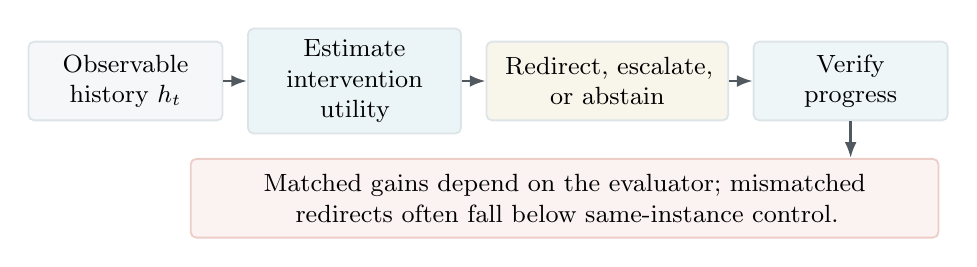
\begin{tikzpicture}[
  node distance=3mm,
  box/.style={draw=PaperGrid, line width=0.65pt, rounded corners=2pt,
              align=center, inner sep=4pt,
              minimum height=10mm, font=\small},
  arrow/.style={-{Latex[length=2mm]}, draw=PaperInk!78, line width=0.9pt},
]
\node[box, fill=PaperGrid!28, text width=0.18\linewidth] (trace)
  {Observable\\history $h_t$};
\node[box, fill=PaperOcean!10, text width=0.20\linewidth, right=of trace] (value)
  {Estimate\\intervention utility};
\node[box, fill=PaperSand!18, text width=0.23\linewidth, right=of value] (control)
  {Redirect, escalate,\\or abstain};
\node[box, fill=PaperOcean!8, text width=0.18\linewidth, right=of control] (verify)
  {Verify\\progress};
\draw[arrow] (trace) -- (value);
\draw[arrow] (value) -- (control);
\draw[arrow] (control) -- (verify);
\node[box, fill=PaperCoral!8, draw=PaperCoral!35,
      text width=0.76\linewidth, below=of value, xshift=0.22\linewidth] (result)
  {Matched gains depend on the evaluator; mismatched redirects often fall below
   same-instance control.};
\draw[arrow] (verify.south) -- (verify.south |- result.north);
\end{tikzpicture}
\caption{\textbf{Selective recovery.} A controller should choose an action by
its expected incremental utility, preserve abstention when evidence is weak, and
verify progress after intervention.  Our current experiments diagnose the
structure--action interaction under privileged context; they do not yet evaluate
the complete loop.}
\label{fig:framework}
\end{figure}


%% ============================================================
%% SECTION 2: RELATED WORK
%% ============================================================
\section{Related Work}

\paragraph{Agent self-correction and repair.}
Reflexion \citep{shinn2023reflexion}, Self-Refine \citep{madaan2023selfrefine}, and self-debugging methods \citep{chen2023teaching, chen2025revisitselfdebugging, olausson2024repair} enable agents to recover from errors through self-generated feedback.
RepairAgent \citep{bouzenia2025repairagent} and AgentCoder \citep{huang2024agentcoder} extend this to multi-step autonomous repair.
Chain-of-thought prompting \citep{wei2022chain}, self-consistency \citep{wang2023selfconsistency}, step-back abstraction \citep{zheng2024stepback}, and decomposed prompting \citep{khot2023decomposed} improve reasoning but do not specifically target recovery from prior errors.
Tree-of-Thought \citep{yao2023tot}, LATS \citep{zhou2024lats}, Agent-R \citep{yuan2025agentr}, and GiGPO \citep{feng2025gigpo} explore recovery through branching, backtracking, or reward-trained policies.
These methods typically evaluate a shared recovery mechanism in aggregate.
We instead hold the mechanism lightweight and ask when its effect changes with
the observable failure category.

\paragraph{Code agent failure analysis.}
SWE-bench \citep{jimenez2024swebench} established the standard evaluation, and systems like SWE-agent \citep{yang2024sweagent}, OpenHands \citep{wang2024openhands}, Agentless \citep{xia2024agentless}, AutoCodeRover \citep{zhang2024autocoderover}, CodeR \citep{chen2024coder}, and MAGIS \citep{tao2024magis} represent the evolving agent landscape.
AgentDebug \citep{zhu2025agentdebug} and MAST \citep{cemri2025mast} categorize failures into stages or communication breakdowns.
SWE-PRM \citep{gandhi2025sweprm} trains a process reward model with type-specific online feedback \citep{lightman2024lets, uesato2022solving}.
\citet{nam2024using} study how LLMs assist code understanding, complementing our focus on failure recovery.
These works motivate failure-aware evaluation.  Our narrower contribution is a
controlled analysis connecting operational failure categories to the effect of
short behavioral redirects.

\paragraph{Trace evidence and test-time control.}
DynaFix \citep{huang2025dynafix}, TraceCoder \citep{huang2026tracecoder}, TraceFixer \citep{bouzenia2023tracefixer}, ARISE \citep{seddik2026arise}, and RGFL \citep{sepidband2026rgfl} condition repair on execution traces, causal analysis, or program graphs.
Test-time scaling and search methods allocate additional computation, whereas
our study concerns a complementary allocation question: when does the observed
history support a low-cost behavioral redirect, and when should a controller
spend more computation on execution evidence or decline to intervene?  This
selective view treats richer repair mechanisms as escalation actions rather
than competitors to a single prompt family.


%% ============================================================
%% SECTION 3: SELECTIVE RECOVERY
%% ============================================================
\section{Selective Recovery as a Control Problem}
\label{sec:formulation}

Let $h_t=(o_1,a_1,\ldots,o_t)$ be the actions and observations available when a
controller considers intervening.  The action set contains abstention
$a_\varnothing$, lightweight redirects such as rereading context or stepping
back, and evidence-seeking escalation such as running targeted tests or
replanning from execution traces.  For an outcome utility $Y$ that combines
task progress with inference and execution cost, the quantity relevant to a
decision is the conditional incremental utility
\begin{equation}
  \Delta(a\mid h_t)
  = \mathbb{E}\!\left[Y(a)-Y(a_\varnothing)\mid h_t\right].
  \label{eq:intervention-utility}
\end{equation}
A selective controller intervenes only when the best supported action has
positive value after accounting for uncertainty and cost; otherwise it
abstains.  Failure-category prediction can inform this estimate, but category
accuracy is not the objective.  Two classifiers with identical accuracy can
have different policy value if one routes its errors to damaging interventions.

This formulation yields three requirements for a deployable evaluation.
First, $h_t$ must exclude the gold patch, gold target files, retrospective
failure labels, and future turns.  Second, detector and action selection must
be frozen on held-out projects so that test outcomes do not choose the policy.
Third, $Y$ must include task-grounded progress, regression risk, and resource
cost rather than prompt compliance alone.  Progress should be checked after an
intervention; a controller can then continue, escalate, or stop instead of
assuming that one redirect repaired the trajectory.

The stored experiments in this paper do not satisfy this complete contract:
they expose gold-derived context and score a single proposed action.  We retain
them because they isolate two quantities that a selective policy must confront:
the apparent upside of a matched redirect and the downside of a mismatch.  We
refer to these results as \emph{oracle-context diagnostics} and avoid treating
them as an evaluation of the full controller in Figure~\ref{fig:framework}.


%% ============================================================
%% SECTION 4: FAILURE TAXONOMY
%% ============================================================
\section{Operational Failure Categories}
\label{sec:taxonomy}

\subsection{Data}

We study 143 failed trajectories from the public O1-agent release on
SWE-bench Verified \citep{jimenez2024swebench}, whose 500 tasks are drawn from
12 Python repositories.\footnote{\url{https://huggingface.co/datasets/AlexCuadron/SWE-Bench-Verified-O1-reasoning-high-results}}
Gold patches are used for retrospective categorization and evaluation; the
analysis therefore concerns failed trajectories rather than leaderboard resolve
rates.
Each trajectory records a sequence of agent actions (file navigation, code edits, command executions) interleaved with environment observations, ranging from 8 to 127 steps with a median of 34.
All trajectories were generated with one agent configuration.  This controls
architectural variation within the dataset but limits generalization to other
agent harnesses.

\subsection{Four categories and behavioral interpretations}

We classify each trajectory with deterministic rules that use tool errors,
patch-application status, and overlap between edited files and the gold patch.
Table~\ref{tab:taxonomy} reports both the implemented criteria and the
behavioral interpretation that motivates each scaffold family.  The
interpretations are hypotheses about observable trajectory structure, not
independently annotated latent reasoning states.

\begin{table}[H]
\centering
\small
\setlength{\tabcolsep}{4pt}
\begin{tabular}{@{}lp{5.0cm}p{3.8cm}r@{}}
\toprule
\textbf{Type} & \textbf{Implemented criterion} & \textbf{Behavioral interpretation} & $\boldsymbol{n}$ \\
\midrule
\textsc{Logic} & Patch applies, task remains unresolved after earlier rules & Diverse but unsuccessful revision & 70 \\[2pt]
\textsc{Loc} & No edited-file overlap with gold patch, or repeated search without edit & Mislocalized effort & 37 \\[2pt]
\textsc{Edit} & Recognized replacement errors dominate before a patch applies & Repetitive retry & 28 \\[2pt]
\textsc{Plan} & Residual after the observable rules above & Plan-level commitment hypothesis & 8 \\
\midrule
\multicolumn{3}{@{}l}{Total} & 143 \\
\bottomrule
\end{tabular}
\caption{Operational failure categories and their motivating behavioral
interpretations. The rules are retrospective because file overlap uses the
gold patch.  We report counts rather than independently rounded percentages.}
\label{tab:taxonomy}
\end{table}

\textsc{Logic} is the largest category (70/143): a patch is applied but the task
remains unresolved after the earlier rules.  We use the literal phrase
\emph{diverse but unsuccessful revision} rather than treating this as an
identified latent reasoning process.  \textsc{Loc} (37/143) denotes either edits
with no file overlap with
the gold patch or repeated search without an edit.  The implementation does not
detect a wrong function inside the correct file.  We interpret the observed
pattern as \emph{mislocalized effort}, while recognizing that exploration
outside the gold files can still be informative.

\textsc{Edit} (28/143) is triggered when failed \texttt{str\_replace} actions
dominate the observable errors.  Repeated variants of the same edit motivate
the \emph{retry-loop} interpretation and a scaffold that refreshes file
context.  \textsc{Plan} (8/143) is the residual category after the three more
directly observable rules.  Its \emph{commitment} interpretation and all
category-level conclusions should be treated cautiously because only eight
trajectories fall in this group.

\subsection{Classification methodology}

The released analysis code applies a deterministic hierarchy.  It assigns
\textsc{Loc} when edited files do not overlap gold-patch files, or when repeated
search produces no edit; \textsc{Edit} when failed replacement operations are
the dominant detected error; \textsc{Logic} when a patch was applied but the
task remained unresolved; and \textsc{Plan} otherwise.  These rules use
retrospective information and are therefore analysis labels, not an online
classifier.  Appendix~\ref{app:classification} states the executable criteria
and their limitations.


%% ============================================================
%% SECTION 4: ERROR CASCADE ANALYSIS
%% ============================================================
\section{Post-Error Tail Analysis}
\label{sec:cascade}

\subsection{Definition}

The annotation script identifies the first \emph{observable environment error}
using a fixed set of error-message patterns.  We summarize where this signal
appears with the post-error tail ratio (PTR):
\begin{equation}
\mathrm{PTR} = \frac{n_{\text{actions at or after first observable error}}}
{n_{\text{actions in the trajectory}}}.
\label{eq:waste}
\end{equation}
PTR is a positional statistic, not a semantic waste annotation: actions in the
tail may still gather useful evidence.  It also misses silent reasoning errors
that produce no recognized environment message.

\subsection{Observable errors often occur early}

Across the 143 failed trajectories, mean PTR is 81.8\% and median PTR is
87.5\%, indicating that the first recognized environment error usually occurs
early in the recorded interaction.  Table~\ref{tab:cascade} gives the
category-level breakdown.

\begin{table}[H]
\centering
\small
\begin{tabular}{@{}lrcc@{}}
\toprule
\textbf{Type} & $\boldsymbol{n}$ & \textbf{Mean PTR (\%)} & \textbf{Interpretation} \\
\midrule
\textsc{Edit} & 28 & 88.8 & Repetitive loops \\
\textsc{Logic} & 70 & 81.2 & Diverse revision \\
\textsc{Loc} & 37 & 80.0 & Mislocalized effort \\
\textsc{Plan} & 8 & 70.7 & Commitment spiral \\
\midrule
All & 143 & 81.8 & --- \\
\bottomrule
\end{tabular}
\caption{Post-error tail ratio by category. PTR is the fraction of recorded
actions at or after the first regex-detected environment error; it does not
label those actions as unproductive.  The overall median is 87.5\%.}
\label{tab:cascade}
\end{table}


PTR alone cannot distinguish repeated retries from diverse revisions.  We
therefore treat the structural labels in Table~\ref{tab:cascade} as hypotheses
motivating the controlled interventions below, rather than as conclusions of
the tail statistic.  The corresponding prediction is that a redirect matched
to a repetitive or reversible pattern should change the proposed next action
more than a redirect applied to the residual \textsc{Logic} category.

%% ============================================================
%% SECTION 5: SCAFFOLDING EXPERIMENTS
%% ============================================================
\section{Oracle-Context Diagnostic Study}
\label{sec:scaffolding}

\subsection{Setup}

The released scripts construct each prompt from the first four recorded turns,
not from an annotated first-error prefix.  To isolate the structure--strategy
interaction, they also provide the gold-derived failure category and gold target
files.  A model then proposes one next action under either a one-sentence
scaffold or a generic retry control.  This is an oracle-context diagnostic
experiment, not an online detection or end-to-end repair experiment.

The automated score ranges from 0 to 3: \emph{file hit} awards one point for
mentioning a gold target-file basename, \emph{actionable} awards one point for a
regex-matched executable step, and \emph{relevant} awards one point for
category-specific recovery language.  Higher is better.  Because target files
appear in the prompt and relevance is lexical, each component is a proxy; the
score measures compliance and next-action specificity rather than patch
correctness.  Appendix~\ref{app:stats} gives the exact rubric and an LLM-judge
sensitivity check.

We test two or three lightweight redirect candidates per category plus control.
These prompts instantiate only the cheapest action family in
\S\ref{sec:formulation}; evidence-seeking escalation and end-to-end verification
are not present in the stored runs.  Primary results use GPT-4o-mini; a smaller
common instance set is repeated across nine models in
\S\ref{sec:cross-model}.  Across matched, mismatched, and cross-model conditions,
the stored outputs contain more than 1,400 scored responses.  Full redirect text
appears in Appendix~\ref{app:prompts}.

\begin{table}[H]
\centering
\small
\setlength{\tabcolsep}{3.5pt}
\begin{tabular}{@{}llccccl@{}}
\toprule
\textbf{Type} & \textbf{Candidate-best} & \textbf{Scaf.} & \textbf{Ctrl} & $\boldsymbol{\Delta}$ & \textbf{95\% CI} & \textbf{Pattern} \\
\midrule
\textsc{Edit} & reread\_file & 2.68 & 1.68 & \textbf{+1.00} & \textbf{[+0.71, +1.32]} & Retry loop \\
\textsc{Plan} & step\_back & 2.75 & 1.88 & \textbf{+0.88} & \textbf{[+0.50, +1.25]} & Commitment \\
\textsc{Loc} & reread\_issue & 1.97 & 1.70 & +0.27 & [$-$0.10, +0.63] & Mislocalized effort \\
\textsc{Logic} & minimal\_fix & 2.13 & 1.97 & +0.17 & [$-$0.07, +0.43] & Diverse revision \\
\bottomrule
\end{tabular}
\caption{Candidate-best scaffold per category under the controlled
next-action protocol (GPT-4o-mini; $n=28,8,30,30$ for \textsc{Edit},
\textsc{Plan}, \textsc{Loc}, and \textsc{Logic}, respectively).  Scores range from 0 to 3;
intervals are paired bootstrap 95\% CIs.  Because the displayed strategy is the
best of two or three candidates, these comparisons are exploratory.}
\label{tab:scaffold-main}
\end{table}

\subsection{Category-conditioned response to redirects}
\label{sec:scaffoldability}

The gains are concentrated in two categories (Table~\ref{tab:scaffold-main}).
For \textsc{Edit}, asking the model to reread the target file raises the reported
score from 1.68 to 2.68 (+1.00).  This is consistent with disrupting a retry
loop, but the one-step protocol cannot show that the subsequent edit succeeds.
For \textsc{Plan}, \emph{step\_back} raises the score by 0.88; this estimate is
promising but imprecise because $n=8$ and the category is residual.

The pattern is weaker for the other categories.  The candidate-best
\textsc{Loc} scaffold gains 0.27 and its interval crosses zero.  The three
\textsc{Logic} candidates cluster near control; the best reported difference is
+0.17.  Within this protocol, short behavioral redirects therefore change the
proxy less for \textsc{Logic} than for \textsc{Edit}.  Richer execution evidence
or multi-step verification is a plausible next test, not a conclusion of these
data.

\paragraph{Held-out selection does not remove evaluator sensitivity.}
Selecting a scaffold on nine projects and evaluating it on the held-out project
retains a +0.44 full-proxy gain over control (95\% project-clustered CI
[+0.33,+0.67], 10 folds).  Thus candidate selection on the evaluation set does
not fully explain the reported full-proxy pattern.  The evaluator does: across
the 96 manuscript-selected pairs, the aggregate gain is +0.50 on the full proxy
but 0.00 (CI [$-$0.09,+0.20]) after removing the type-specific relevance term;
the actionable-only difference is $-$0.14 (CI [$-$0.21,+0.06]).  On the 37 pairs
covered by the stored blinded LLM judge, the regex difference is +0.65 but the
judge difference is +0.14 (CI [$-$0.16,+0.24]).  The large matched gains should
therefore be interpreted as scaffold--evaluator alignment, not
evaluator-independent next-action improvement
(Figure~\ref{fig:cross-type-transfer}a).

\paragraph{Qualitative audit exposes proxy shortcuts.}
The stored responses make the measurement problem concrete.  On
\texttt{django\_\_django-11885}, \emph{reread\_file} emits a command that displays
the disclosed target file and receives 3/3, whereas control runs the issue's
reproduction script and receives 0/3.  The former follows the prompt more
literally, but the latter may still provide useful execution evidence.  On
\texttt{sphinx-doc\_\_sphinx-10323}, \emph{minimal\_fix} emits the placeholder
substitution \texttt{old\_logic/new\_logic} and nevertheless receives 3/3.  These
are not claims that either action repairs the issue; they show how file mention,
command form, and category words can reward compliance without semantic
progress.  This motivates task-grounded verification in
Eq.~\ref{eq:intervention-utility}.

\paragraph{Mismatched redirects often reduce the proxy.}
For \textsc{Loc}, \emph{test\_guided} scores 0.87 versus 1.70 for control, a
0.83-point decrease.  Pairing every cross-category response with the same
instance's control yields negative means for 10 of 12 off-diagonal pairs on the
full proxy and 11 of 12 without the relevance term
(Figure~\ref{fig:cross-type-transfer}b; Table~\ref{tab:cross-type}).  Only three
project-clustered intervals lie fully below zero, so the pair-specific estimates
remain uncertain.  Nevertheless, the direction is more stable than the matched
gain under evaluator ablation.  The result is descriptive of the tested prompt
set; it does not establish that every mismatched recovery strategy is harmful.

\begin{figure}[t]
\centering
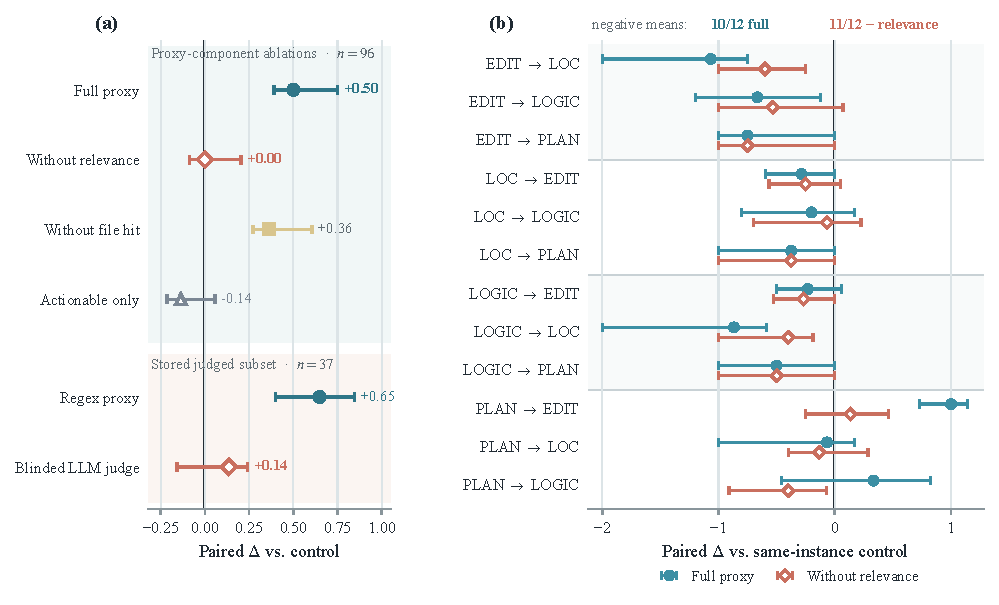
\includegraphics[width=0.98\columnwidth]{figure2_experiment_summary.pdf}
\caption{\textbf{Evaluator sensitivity and paired negative transfer.}
(a) The matched gain is large on the full regex proxy but vanishes without its
type-lexical relevance component and is small under the stored blinded judge
($n=96$; judged subset $n=37$).
(b) Cross-category responses are paired with the same instance's control; 10 of
12 full-proxy means and 11 of 12 means without relevance are negative, although
only three intervals in each specification exclude zero.  Bars in both panels
are 95\% project-clustered bootstrap intervals.}
\label{fig:cross-type-transfer}
\end{figure}

\subsection{Oracle category-conditioned selection as headroom}
\label{sec:strategy-selection}

We compare an oracle that chooses the candidate-best scaffold using the
gold-derived category, a fixed \emph{reread\_file} scaffold, and control.  This
analysis quantifies headroom under privileged context; it is not a deployable
routing evaluation.

\begin{table}[H]
\centering
\small
\setlength{\tabcolsep}{4pt}
\begin{tabular}{@{}lccc@{}}
\toprule
\textbf{Condition} & \textbf{Score} & \textbf{File Hit} & \textbf{Score $\boldsymbol{\Delta}$} \\
\midrule
Oracle (category-specific) & 2.33 & 83\% & +0.57 \\
Fixed (reread\_file) & 2.04 & 75\% & +0.28 \\
Control (no scaffold) & 1.76 & 72\% & --- \\
\bottomrule
\end{tabular}
\caption{Oracle-context strategy comparison on 96 stored instances.  The
oracle uses the gold-derived category and selects the best candidate on the
same evaluation set; its 2.33 score is therefore an optimistic upper bound.}
\label{tab:strategy-selection}
\end{table}

The reported oracle score is 2.33, compared with 2.04 for the fixed scaffold and
1.76 for control.  Its advantage is partly selected on the evaluation set and
thus should be read as evidence that scaffold effects differ by category, not
as an unbiased estimate of a learned router.  A deployable test requires a
strictly observable classifier, held-out strategy selection, and prompts that
omit gold category and target files.

\subsection{Cross-Model Analysis}
\label{sec:cross-model}

We repeat one matched scaffold and control on a common subset for nine models
from four families.  This checks whether the small \textsc{Logic} effect is
specific to GPT-4o-mini, while retaining all limitations of the proxy protocol.
Figure~\ref{fig:heatmap} visualizes the differences and
Table~\ref{tab:cross-model} reports the full matrix.

\begin{table}[H]
\centering
\small
\begin{tabular}{@{}llrrrrrrrr@{}}
\toprule
& & \multicolumn{2}{c}{\textbf{\textsc{Edit}}} & \multicolumn{2}{c}{\textbf{\textsc{Loc}}} & \multicolumn{2}{c}{\textbf{\textsc{Logic}}} & \multicolumn{2}{c}{\textbf{\textsc{Plan}}} \\
\cmidrule(lr){3-4}\cmidrule(lr){5-6}\cmidrule(lr){7-8}\cmidrule(lr){9-10}
\textbf{Model} & \textbf{Tier} & \textbf{Ctrl} & $\boldsymbol{\Delta}$ & \textbf{Ctrl} & $\boldsymbol{\Delta}$ & \textbf{Ctrl} & $\boldsymbol{\Delta}$ & \textbf{Ctrl} & $\boldsymbol{\Delta}$ \\
\midrule
GPT-4o-mini & mid & 1.61 & +1.04 & 1.54 & +0.49 & 2.01 & +0.13 & 1.88 & +0.88 \\
DS-V4-Flash & mid & 2.27 & +0.60 & 2.00 & +0.40 & 2.33 & +0.13 & 1.88 & +0.63 \\
Qwen 3.5 & mid & 2.40 & +0.00 & 2.13 & +0.13 & 2.33 & +0.07 & 1.62 & +1.38 \\
\midrule
DS-V4-Pro & strong & 1.53 & +0.73 & 1.67 & +0.87 & 2.33 & +0.07 & 1.88 & $-$0.38 \\
GPT-4.1 & strong & 1.80 & +0.60 & 2.27 & $-$0.20 & 2.33 & 0.00 & 1.88 & $-$0.38 \\
Claude Son.\ 4.6 & strong & 2.79 & $-$0.07 & 2.50 & +0.13 & 2.50 & 0.00 & 2.00 & +0.12 \\
\midrule
Claude Opus 4.7 & frontier & 2.27 & +0.13 & 2.47 & +0.27 & 2.40 & +0.13 & 2.00 & 0.00 \\
o4-mini$^\dagger$ & frontier & 1.53 & +0.53 & 0.93 & +1.47 & 1.33 & $-$0.20 & 1.75 & +0.38 \\
GPT-5.5$^\dagger$ & frontier & 1.00 & +1.20 & 0.80 & +1.60 & 1.60 & $-$0.40 & 1.60 & $-$0.20 \\
\bottomrule
\end{tabular}
\caption{Scaffold effect ($\Delta$) across nine models under the same
oracle-context next-action protocol. $^\dagger$Reasoning-chain models.  The
\textsc{Logic} column ranges from $-$0.40 to +0.13; other categories show mixed,
model-dependent effects.}
\label{tab:cross-model}
\end{table}

\begin{figure}[!htbp]
\centering
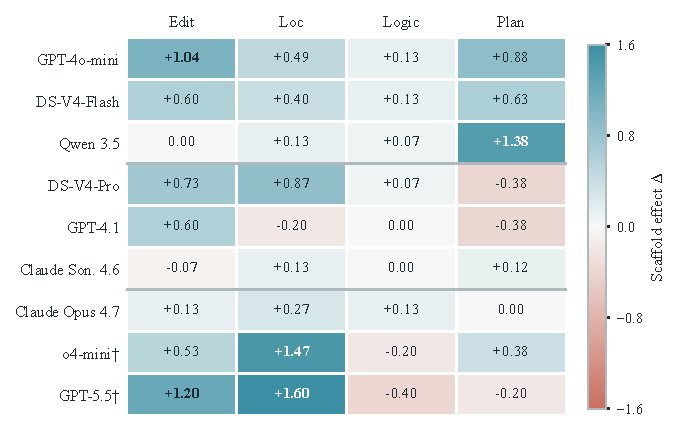
\includegraphics[width=0.84\columnwidth]{figure3_cross_model_heatmap.pdf}
\caption{\textbf{Cross-model scaffold effects.} The heatmap uses oracle
diagnostic context.  The
continuous diverging scale is centered at zero, and horizontal rules separate
the mid, strong, and frontier tiers in Table~\ref{tab:cross-model}.  The
\textsc{Logic} differences are small or negative for all nine models; effects in
the other columns vary across models.}
\label{fig:heatmap}
\end{figure}

The \textsc{Logic} effect remains small or negative for every model (range
$-$0.40 to +0.13), making this the most consistent cross-model observation.
\textsc{Edit} is positive for seven of nine models, but the magnitude varies
from $-$0.07 to +1.20.  \textsc{Loc} and \textsc{Plan} are less stable: both
contain negative cells and large positive cells.  These mixed results argue
against a universal redirect.  They also show that the current study cannot
separate category structure from model-specific prompt sensitivity.  Because
this matrix uses the full regex proxy, it should be read as a cross-model prompt
compliance diagnostic rather than independent validation of recovery quality.


%% ============================================================
%% SECTION 6: DISCUSSION
%% ============================================================
\FloatBarrier
\section{Discussion}
\label{sec:discussion}

\paragraph{The main design consequence is selective intervention.}
A redirect can strongly change lexical and target-following behavior, but its
matched advantage does not survive removal of the relevance component or the
blinded-judge check.  Negative off-diagonal transfer is more common across
proxy specifications.  A recovery controller should therefore estimate the
value of a particular action, not merely detect that a failure occurred.  When
evidence for a cheap redirect is weak, abstention or evidence-seeking escalation
is preferable to forced routing.

\paragraph{The majority category needs evidence, not stronger slogans.}
The applied-but-unresolved \textsc{Logic} group contains 70 of 143 trajectories,
and short redirects remain near zero across nine models under the current
proxy.  This observation does not define a universal frontier for behavioral
intervention: the prompt set is small and the category is coarse.  It instead
prioritizes a stronger comparison between one-sentence redirects and actions
that obtain new information, such as targeted test analysis, trace-conditioned
replanning, or process-level verification.  In the selective-recovery action
space, these are escalation policies rather than more elaborate phrasings of
the same scaffold.

\paragraph{Policy value should replace classifier accuracy.}
A simple four-way router maps a retrospective category to a fixed prompt.  This
decomposition is useful for analysis but too rigid for deployment.  A
controller can have high category accuracy and still reduce task success if its
few errors select harmful redirects.  Conversely, a calibrated policy that
intervenes on a small set of clear retry loops may have higher utility despite
lower coverage.  Evaluation should therefore report risk--coverage curves,
intervention harm, task success, and cost, together with category metrics used
only for diagnosis.

\paragraph{What remains to establish recovery.}
The present evidence does not justify a deployed architecture.  The diagnostic
prompts expose category and target files, the candidate-best redirect is chosen
using evaluation outcomes, and the score does not verify a patch.  A decisive
test must infer action value from prefix-only observations, freeze routing and
redirect selection on held-out projects, resume the repository agent under a
fixed budget, and verify tests and regressions.  Under that design, the present
results supply intervention candidates, failure cases, and a risk-sensitive
decision objective rather than performance guarantees.


%% ============================================================
%% ============================================================
%% SECTION 7: CONCLUSION
%% ============================================================
\section{Conclusion}

Code-agent recovery should be treated as selective control, not an automatic
retry.  Our audit of 143 failed trajectories and more than 1,400 controlled
responses finds that apparent benefits of matched redirects are strongly
evaluator-sensitive, while negative transfer from mismatched redirects is more
persistent.  The appropriate deployment objective is therefore incremental
task utility under cost and uncertainty: redirect when evidence supports a
specific low-cost action, escalate when new execution evidence is needed, and
abstain when neither is justified.  Establishing this policy requires
prefix-only decisions and end-to-end repository verification; the current
oracle-context study defines the risks and evaluation contract for that test.

%% ============================================================
%% LIMITATIONS (does not count toward page limit)
%% ============================================================
\section*{Limitations}

The dataset contains failed trajectories from one agent configuration on Python
repositories in SWE-bench Verified, so category prevalence need not transfer to
other harnesses, languages, or successful runs.  Categories use gold-patch
overlap retrospectively, and \textsc{Plan} is a small residual group ($n=8$).
The behavioral interpretations are not independently annotated structural
measurements, and the current implementation detects localization only at file
level rather than wrong-function edits within a correct file.

The intervention prompts contain the gold-derived category and target files and
use the first four recorded turns rather than a synchronized first-error prefix.
The outcome is one generated action scored by lexical proxies; target-file hit
is especially easy because the target is disclosed.  The experiment therefore
does not measure repair success, cost, or multi-turn side effects.  Candidate-best
strategies are selected from two or three prompts on the evaluation categories,
although leave-one-project-out selection retains a full-proxy gain.  More
importantly, the matched gain vanishes when the type-lexical relevance component
is removed and is small on the incomplete blinded-judge subset.  Cross-model
results reuse the full proxy and should not be interpreted as independent
end-to-end validation.

The qualitative audit is illustrative rather than a substitute for blinded
human assessment.  The stored LLM-judge subset is incomplete, and the paper does
not claim inter-annotator agreement because the corresponding manual-label
artifact is unavailable.  Human evaluation remains useful for
validating next-action semantics, but it cannot replace repository tests as the
primary recovery outcome.

Selective intervention could reduce unnecessary model calls and developer
waiting time if validated in a real agent loop.  Conversely, a mistimed
controller could suppress useful exploration or steer an agent toward an
incorrect repository change.  The present proxy study is not sufficient for
deployment in safety-critical software workflows.


\bibliographystyle{plainnat}
\bibliography{references}

%% ============================================================
%% APPENDIX
%% ============================================================
\appendix

\section{Prompt Templates}
\label{app:prompts}

All scaffold prompts are short directives appended after the first four recorded
turns.  The surrounding template states the gold-derived failure category and
gold target files.  The control receives a generic retry instruction (``try
again with a different approach'') under the same diagnostic context.  Below we
reproduce the scaffold-specific sentence.

\subsection{\textsc{Edit} Strategies}

\paragraph{reread\_file:} ``Before attempting the edit again, re-read the target file to refresh your understanding of its current contents.''

\paragraph{smaller\_edit:} ``Try breaking your edit into smaller, more targeted changes rather than replacing a large block at once.''

\subsection{\textsc{Plan} Strategies}

\paragraph{step\_back:} ``Step back and re-read the original issue description. Reconsider whether your current approach is the right way to address what is being asked.''

\paragraph{scope\_check:} ``Verify that the scope of your current changes matches what the issue is actually requesting.''

\subsection{\textsc{Loc} Strategies}

\paragraph{reread\_issue:} ``Re-read the original issue description carefully and identify any clues about which specific file or function is responsible for the reported behavior.''

\paragraph{test\_guided:} ``Run the relevant test suite to identify which component is actually failing, and use that to guide your search for the right file to modify.''

\paragraph{broaden\_search:} ``Stop working on your current target file. Search more broadly. Check related modules, imported files, and parent classes. Trace the symptoms to a different code location.''

\subsection{\textsc{Logic} Strategies}

\paragraph{minimal\_fix:} ``Focus on making the smallest possible change that addresses the core issue, rather than a comprehensive rewrite.''

\paragraph{test\_analysis:} ``Analyze the failing test assertion carefully. What exact value or behavior does it expect? Compare against what your code produces, and identify the specific computation your fix gets wrong.''

\paragraph{edge\_cases:} ``Your fix may address the common case but miss edge cases that the test exercises. Consider boundary conditions (empty inputs, zero, negative values) and re-read the test to identify which case it targets.''


\section{Detailed Strategy Results}
\label{app:per-instance}

Tables~\ref{tab:per-instance-edit}--\ref{tab:per-instance-logic} report aggregate
score components for all strategies and the control condition.

\begin{table}[H]
\centering
\small
\begin{tabular}{@{}lcccc@{}}
\toprule
\textbf{Metric} & \textbf{reread} & \textbf{smaller} & \textbf{control} \\
\midrule
Mean Score & 2.68 & 1.86 & 1.68 \\
File Hit (\%) & 89 & 89 & 75 \\
Actionable (\%) & 100 & 96 & 89 \\
Relevant (\%) & 79 & 0 & 4 \\
\bottomrule
\end{tabular}
\caption{Strategy comparison for \textsc{Edit} failures ($n=28$, GPT-4o-mini).}
\label{tab:per-instance-edit}
\end{table}

\begin{table}[H]
\centering
\small
\begin{tabular}{@{}lcccc@{}}
\toprule
\textbf{Metric} & \textbf{step\_back} & \textbf{scope} & \textbf{control} \\
\midrule
Mean Score & 2.75 & 1.88 & 1.88 \\
File Hit (\%) & 100 & 88 & 88 \\
Actionable (\%) & 88 & 100 & 100 \\
Relevant (\%) & 88 & 0 & 0 \\
\bottomrule
\end{tabular}
\caption{Strategy comparison for \textsc{Plan} failures ($n=8$, GPT-4o-mini).}
\label{tab:per-instance-plan}
\end{table}

\begin{table}[H]
\centering
\small
\setlength{\tabcolsep}{3pt}
\begin{tabular}{@{}lcccc@{}}
\toprule
\textbf{Metric} & \textbf{reread} & \textbf{test\_g.} & \textbf{broaden} & \textbf{ctrl} \\
\midrule
Mean Score & 1.97 & 0.87 & 1.93 & 1.70 \\
File Hit (\%) & 73 & 23 & 87 & 53 \\
Actionable (\%) & 23 & 63 & 70 & 83 \\
Relevant (\%) & 100 & 0 & 37 & 33 \\
\bottomrule
\end{tabular}
\caption{Strategy comparison for \textsc{Loc} failures ($n=30$, GPT-4o-mini).
test\_g.\ denotes test\_guided, which scores 0.83 below control.}
\label{tab:per-instance-loc}
\end{table}

\begin{table}[H]
\centering
\small
\setlength{\tabcolsep}{3pt}
\begin{tabular}{@{}lcccc@{}}
\toprule
\textbf{Metric} & \textbf{min\_fix} & \textbf{test\_a.} & \textbf{edge\_c.} & \textbf{ctrl} \\
\midrule
Mean Score & 2.13 & 2.07 & 2.07 & 1.97 \\
File Hit (\%) & 90 & 87 & 90 & 83 \\
Actionable (\%) & 100 & 80 & 83 & 90 \\
Relevant (\%) & 23 & 40 & 33 & 23 \\
\bottomrule
\end{tabular}
\caption{Strategy comparison for \textsc{Logic} failures ($n=30$,
GPT-4o-mini). All strategy means lie within 0.16 points of one another.}
\label{tab:per-instance-logic}
\end{table}


\section{Statistical Methods}
\label{app:stats}

\paragraph{Bootstrap confidence intervals.}
For Table~\ref{tab:scaffold-main}, we align scaffold and control scores by
instance, resample the paired differences with replacement 10,000 times, and
report the 2.5th and 97.5th percentiles.  The local audit script uses a fixed
random seed and reproduces the four displayed intervals.

\paragraph{Selection and multiple comparisons.}
The strategy shown for each category is the largest observed mean among two or
three candidates, and the oracle reuses this selection.  The bootstrap intervals
condition on the selected candidate and are not adjusted for selection or
multiple comparisons.  We therefore treat these results as exploratory and do
not make statistical-significance claims from them.

\paragraph{Project-held-out selection.}
We group instances by their source project.  For each of 10 folds, candidate
means are computed on the other nine projects, one scaffold is selected per
category, and its stored response is evaluated on the held-out project.  The
resulting 96 paired differences are summarized with a project-clustered
percentile bootstrap (10,000 resamples, fixed seed).  This yields 2.229 for the
selected scaffold versus 1.792 for control, $\Delta=+0.438$ with 95\% CI
[+0.333,+0.674].

\paragraph{Proxy ablations.}
Using the same manuscript-selected scaffold for each category, the aggregate
paired difference is +0.500 [+0.393,+0.750] on the full proxy, 0.000
[$-$0.088,+0.204] without type-specific relevance, +0.365
[+0.273,+0.605] without file hit, and $-$0.135 [$-$0.213,+0.059] for
actionability alone.  Intervals resample source projects and therefore reflect
cross-project rather than generation-seed variability.

\paragraph{Effect sizes.}
All reported $\Delta$ values are paired mean differences on the 0--3 scoring
scale.  We report this native unit rather than a standardized effect because the
three-point total is discrete and its components are heterogeneous.

\paragraph{Automated scoring rubric.}
Scoring is automated via pattern matching on model outputs.
\textit{File hit} (1 point): the response references the correct target file (identified by basename matching against the reference solution).
\textit{Actionable} (1 point): the response matches a regex for executable commands or code edits (e.g., \texttt{cat}, \texttt{grep}, \texttt{python}, \texttt{str\_replace}).
\textit{Relevant} (1 point): type-specific regex detects appropriate recovery behavior, e.g., for \textsc{Edit}, terms like ``read,'' ``view,'' ``exact,'' ``whitespace''; for \textsc{Plan}, terms like ``approach,'' ``alternative,'' ``reconsider.''
The rubric is reproducible but lexically biased: a response can earn relevance
by echoing scaffold vocabulary without improving a patch.
We therefore compare it with two stored LLM-judge evaluations; these are
sensitivity analyses, not human validation.
First, GPT-4.1 judged 60 sampled responses (15 per type) with access to gold files and failure-type context; within-$\pm$1 agreement was 95\% (57/60).
Second, we expanded to 220 responses using a \textit{blinded} GPT-4o-mini judge that received no type-specific keywords in its rubric, only ``file relevant,'' ``actionable,'' and ``progress'' dimensions.
On this blinded evaluation, within-$\pm$1 agreement is 82\%.  Only 37 responses
form matched scaffold--control pairs for the manuscript-selected strategies.
On this paired subset, the regex difference is +0.649
[+0.400,+0.846], whereas the blinded-judge difference is +0.135
[$-$0.158,+0.240].  This discrepancy reinforces the need to interpret the full
proxy as lexical compliance rather than evaluator-independent action quality.

\paragraph{File-hit sensitivity analysis.}
Removing the type-specific relevance component leaves a simpler binary outcome:
whether the response mentions a gold target-file basename.  Table~\ref{tab:filehit-robustness}
shows that the direction of several effects remains visible.  However, this is
not an independent correctness measure because the prompt itself discloses the
target files; it measures whether the model follows that supplied context.

\begin{table}[H]
\centering
\small
\begin{tabular}{@{}llcccc@{}}
\toprule
\textbf{Type} & \textbf{Strategy} & \textbf{Hit} & \textbf{Ctrl} & $\boldsymbol{\Delta}$ \textbf{(pp)} & $\boldsymbol{p}$ \\
\midrule
\textsc{Edit} & reread\_file & 89\% & 75\% & +14 & 0.30 \\
\textsc{Plan} & step\_back & 100\% & 88\% & +13 & 1.00 \\
\textsc{Loc} & broaden & 87\% & 53\% & +33 & 0.01$^*$ \\
\textsc{Logic} & minimal\_fix & 90\% & 83\% & +7 & 0.71 \\
\midrule
\textsc{Loc} & test\_guided & 23\% & 53\% & $-$30 & 0.03$^*$ \\
\bottomrule
\end{tabular}
\caption{Target-file mention rates by category and strategy.  The outcome has no
type-specific relevance regex, but the gold target files are supplied in the
prompt, so it should be interpreted as context-following rather than repair
correctness.  Reported Fisher tests are uncorrected descriptive analyses.}
\label{tab:filehit-robustness}
\end{table}

\paragraph{Cross-model experiment details.}
All nine models were evaluated on the same instance set (15 per type for \textsc{Edit}/\textsc{Loc}/\textsc{Logic}, 8 for \textsc{Plan}), yielding 53 scored responses per model per condition.
API calls used temperature 0 for standard models and default settings for reasoning-chain models ($^\dagger$), accessed via a unified API proxy between April--May 2026.
All models received the same prompt construction, including gold-derived
category and target-file context.


\section{Classification Methodology Details}
\label{app:classification}

\subsection{Hierarchical Classification Rules}

The released annotation script proceeds through the following decision tree:

\begin{enumerate}
\item \textbf{Localization}: assign \textsc{Loc} if at least one edit occurs
but no edited path overlaps a gold-patch path, or if the trajectory contains no
edit and at least three search actions.
\item \textbf{Edit application}: assign \textsc{Edit} after at least two
recognized replacement errors, or after one replacement error when no patch was
applied and replacement errors constitute at least half of detected errors.
\item \textbf{Applied patch}: assign \textsc{Logic} when the harness records
that a patch was applied but the instance remains failed.
\item \textbf{Residual rules}: the code next checks repeated test errors,
long correct-file trajectories, and search-heavy behavior; remaining cases are
assigned \textsc{Plan}.  No trajectory in the analyzed file receives the
intermediate \textsc{Test} label.
\end{enumerate}

The hierarchy is intentionally pragmatic rather than ontological.  In
particular, \textsc{Plan} is a fallback, and both file overlap and patch status
depend on retrospective benchmark artifacts.  The repository does not contain
a manual-label artifact, so we do not report an inter-annotator agreement claim.
Likewise, stored online-classifier summaries are internally inconsistent with
the available confusion matrix and lack the training script and per-instance
predictions; online routing results are omitted from this version.

\section{Paired Cross-Category Transfer}
\label{app:cross-type}

Table~\ref{tab:cross-type} reports 183 stored cross-category evaluations.  Each
response is paired with its own instance's control, avoiding the earlier
comparison between subset scaffold means and category-wide control means.  Ten
of twelve full-proxy means are negative; 11 of 12 are negative when the
type-lexical relevance component is removed.  Only three intervals in each
specification lie fully below zero.

\begin{table}[H]
\centering
\scriptsize
\setlength{\tabcolsep}{3.2pt}
\begin{tabular}{@{}llrcc@{}}
\toprule
\textbf{Source} & \textbf{Target} & $\boldsymbol{n}$ & \textbf{Full $\Delta$ [95\% CI]} & \textbf{No-rel. $\Delta$ [95\% CI]} \\
\midrule
\textsc{Edit} & \textsc{Loc} & 15 & $-$1.07 [$-$2.00,$-$0.75] & $-$0.60 [$-$1.00,$-$0.25] \\
\textsc{Edit} & \textsc{Logic} & 15 & $-$0.67 [$-$1.20,$-$0.13] & $-$0.53 [$-$1.00,+0.07] \\
\textsc{Edit} & \textsc{Plan} & 8 & $-$0.75 [$-$1.00,0.00] & $-$0.75 [$-$1.00,0.00] \\
\midrule
\textsc{Loc} & \textsc{Edit} & 28 & $-$0.29 [$-$0.59,0.00] & $-$0.25 [$-$0.57,+0.05] \\
\textsc{Loc} & \textsc{Logic} & 15 & $-$0.20 [$-$0.80,+0.17] & $-$0.07 [$-$0.70,+0.23] \\
\textsc{Loc} & \textsc{Plan} & 8 & $-$0.38 [$-$1.00,0.00] & $-$0.38 [$-$1.00,0.00] \\
\midrule
\textsc{Logic} & \textsc{Edit} & 26 & $-$0.23 [$-$0.50,+0.06] & $-$0.27 [$-$0.53,0.00] \\
\textsc{Logic} & \textsc{Loc} & 15 & $-$0.87 [$-$2.00,$-$0.58] & $-$0.40 [$-$1.00,$-$0.19] \\
\textsc{Logic} & \textsc{Plan} & 8 & $-$0.50 [$-$1.00,0.00] & $-$0.50 [$-$1.00,0.00] \\
\midrule
\textsc{Plan} & \textsc{Edit} & 15 & +1.00 [+0.73,+1.14] & +0.13 [$-$0.25,+0.46] \\
\textsc{Plan} & \textsc{Loc} & 15 & $-$0.07 [$-$1.00,+0.17] & $-$0.13 [$-$0.40,+0.29] \\
\textsc{Plan} & \textsc{Logic} & 15 & +0.33 [$-$0.45,+0.82] & $-$0.40 [$-$0.91,$-$0.07] \\
\bottomrule
\end{tabular}
\caption{Paired off-diagonal transfer.  No-rel. removes the type-specific
relevance point from both scaffold and control scores.  Intervals are 95\%
project-clustered percentile-bootstrap intervals with 10,000 resamples.}
\label{tab:cross-type}
\end{table}


\FloatBarrier
\input{checklist}

\end{document}
